\documentclass[a4paper]{article}

\usepackage{INTERSPEECH2021}
\usepackage{booktabs}
\usepackage{graphicx}

% Align floats on a float page to the top instead of vertically centered
\makeatletter
\setlength{\@fptop}{0pt}
\makeatother

\title{NLU course project: Language Modeling}
\name{Elena Deidda (mat. 267887)}

\address{
  University of Trento}
\email{elena.deidda@studenti.unitn.it}

\begin{document}

\maketitle

\section{Introduction}
I tackle word-level language modeling on the Penn TreeBank corpus, evaluated
with perplexity (PPL). In Part~A I train a GPT-2-style decoder-only
Transformer~\cite{vaswani2017} \emph{from scratch}, improving it step by step
through learning-rate and architecture search, dropout and a weight-tying
ablation, lowering the test PPL from 35.68 to 33.07. In Part~B I fine-tune the
\emph{pre-trained} GPT-2 with a hand-implemented LoRA, training only low-rank
adapters on the $Q,K,V$ projections while the 124M backbone stays frozen,
reaching test PPL 19.14. Both parts satisfy PPL${<}250$, and Part~B clearly
benefits from starting from a pre-trained model.

\section{Implementation details}
Sentences are tokenized with the GPT-2 BPE tokenizer and padded on the right
(padding ignored in the loss); PPL is the exponential of the per-token
cross-entropy. Every experiment follows a greedy, one-change-at-a-time search,
selected on \emph{dev} PPL, with AdamW, gradient clipping and early stopping.

\textbf{Part A.} Search order: learning rate (on the smallest model), then the
architecture one hyper-parameter at a time (\texttt{d\_model}, heads, layers,
FFN size), then dropout, then a weight-tying ablation
(\texttt{lm\_head} tied to the token embedding)~\cite{press2017}. Tying did
\emph{not} help here: the tied model needed 20 epochs to converge against 7
for the untied one, and reached a worse PPL despite ${\sim}19$M fewer
parameters, so I keep the untied model as final. The fact that the tied model
needs almost three times as many epochs to converge, while still reaching a
worse PPL, suggests that the constraint makes optimization harder (conflicting
gradients between the embedding and output-projection roles) more than the
parameter reduction helps generalization -- an effect likely tied to the
combination of a pre-norm Transformer architecture and a small training
corpus, unlike the LSTM setting of the original weight-tying study.

\textbf{Part B.} LoRA~\cite{hu2022} is implemented manually: each attention
layer injects low-rank matrices $A,B$ into $Q,K,V$, computing
$\Delta Wx=(\alpha/r)BAx$. $A\sim\mathcal{N}(0,1)$, $B$ is zero-initialized, so
training starts exactly from the pre-trained model; only the adapters train
(0.7\% of parameters at rank 16). HuggingFace's internal label shifting is
used, so labels are not shifted manually as in Part~A. Search order: learning
rate (rank 4, $\alpha{=}8$ fixed), then rank $r\in\{4,8,16\}$ ($\alpha{=}2r$),
then $\alpha$ at the best rank.

\section{Results}
Models are selected on dev PPL and scored on test PPL. Table~\ref{tab:lma} and
Figure~\ref{fig:lma} trace Part~A: every step except weight tying improves
test PPL. Within the architecture step, doubling \texttt{n\_heads} (4$\to$8)
helped at no parameter cost, while halving \texttt{num\_layers} (4$\to$2)
clearly hurt (test PPL 37.57, not shown). Table~\ref{tab:lmb} reports Part~B:
PPL decreases monotonically with rank, and a smaller-than-default scaling
($\alpha{=}8$ at rank 16) gives the best result, test PPL 19.14 -- a 42\%
relative improvement over the best from-scratch model while training only
0.88M of 125M parameters.

\begin{figure}[t]
  \centering
  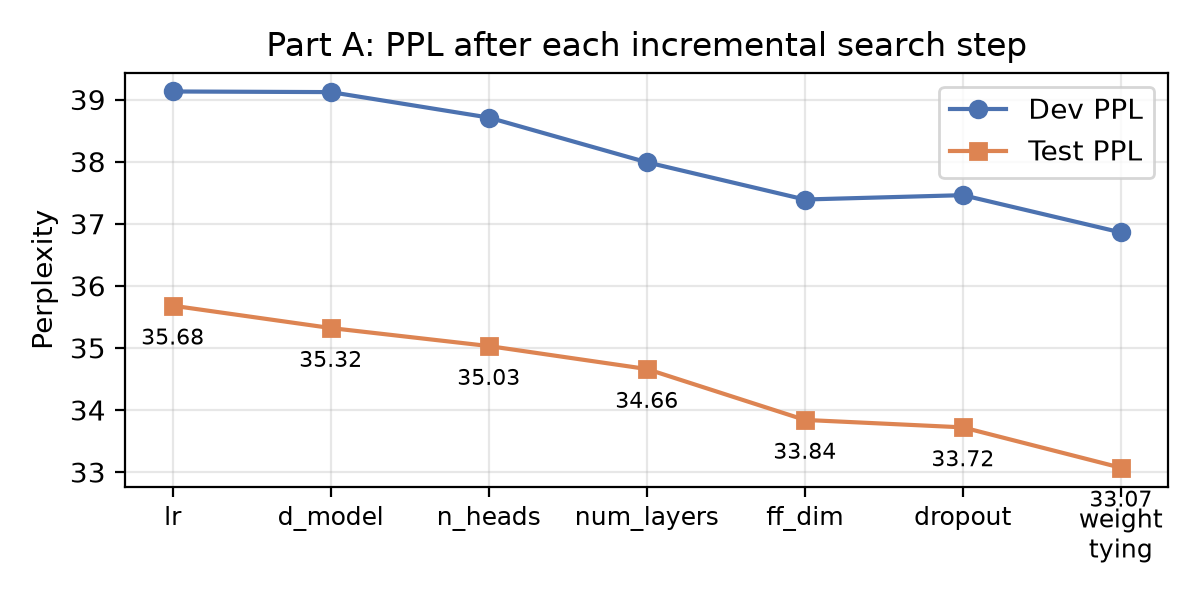
\includegraphics[width=\linewidth]{partA_ppl_steps.png}
  \caption{Part~A: dev and test PPL after each incremental search step.}
  \label{fig:lma}
\end{figure}

\begin{table}[t]
  \centering
  \caption{Part~A --- best model per step. Final: $d{=}384$, 8 heads,
           6 layers, FFN 2048, dropout 0.1, no weight tying.}
  \label{tab:lma}
  \begin{tabular}{llrrr}
    \toprule
    Step & Config & Param & Dev & Test \\
    \midrule
    0 -- lr            & $5{\cdot}10^{-4}$ & 29.2M & 39.13 & 35.68 \\
    1.1 -- d\_model    & $384$             & 44.6M & 39.12 & 35.32 \\
    1.2 -- heads       & $8$               & 44.6M & 38.71 & 35.03 \\
    1.3 -- layers      & $6$               & 47.3M & 37.99 & 34.66 \\
    1.4 -- FFN         & $2048$            & 52.1M & 37.39 & 33.84 \\
    2 -- dropout       & $0.1$             & 52.1M & 37.46 & 33.72 \\
    3 -- weight tying  & not tied          & 52.1M & \textbf{36.86} & \textbf{33.07} \\
    \bottomrule
  \end{tabular}
\end{table}

\begin{table}[t]
  \centering
  \caption{Part~B --- LoRA fine-tuning ($lr{=}5{\cdot}10^{-4}$). 124.4M
           backbone frozen throughout.}
  \label{tab:lmb}
  \begin{tabular}{rrrrr}
    \toprule
    Rank $r$ & $\alpha$ & Train. & Dev & Test \\
    \midrule
    4  & 8  & 0.22M & 23.27 & 21.02 \\
    8  & 16 & 0.44M & 21.99 & 19.91 \\
    16 & 32 & 0.88M & 21.20 & 19.35 \\
    16 & 8  & 0.88M & \textbf{21.03} & \textbf{19.14} \\
    \bottomrule
  \end{tabular}
\end{table}

\bibliographystyle{IEEEtran}
\bibliography{mybib}

\end{document}
